% arara: pdflatex

\documentclass[tikz,border=0pt]{standalone}
\usepackage{pgfplots}
\usepackage{xcolor}
\usepackage{siunitx}
\usepgflibrary{arrows, shadings}

\definecolor{summersky}{RGB}{51,204,255}
\definecolor{groen}{rgb}{0.0, 0.5, 0.0}
\begin{document}

\begin{tikzpicture}
% width is 8.64cm
\newcommand{\figwidth}{9.20cm}
%\newcommand{\figwidth}{17.80cm}
\newcommand{\figheight}{5.33cm}

\draw[use as bounding box, white] (0,0) rectangle (\figwidth,\figheight);


% A) Oil Description
\begin{scope}[
    xshift=2.9cm,
    yshift=2.8cm,
    ]
    \node[inner sep=0pt]  at (0,0)
        {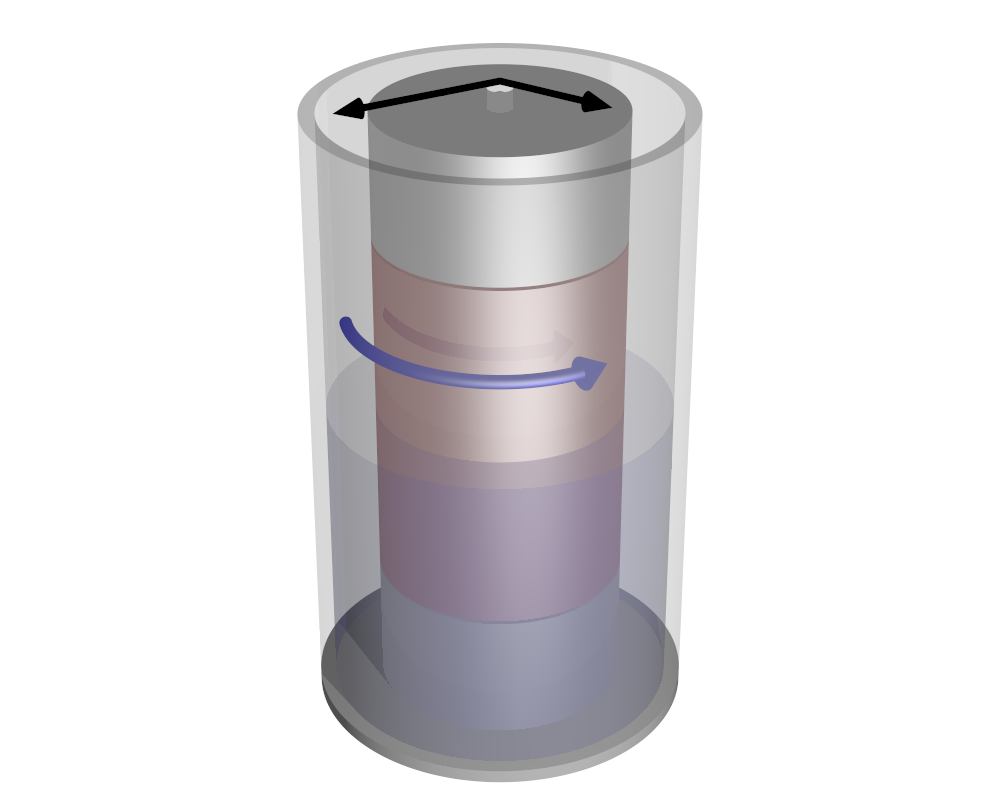
\includegraphics[
            height=5.60cm,
            trim={5cm, 0.25cm, 3.8cm, 0},
            clip
        ]{t3csetup.png}};

    \node at (-0.2, 0.4) {\Large$\omega_i$};
        \node at (0.3, 2.35) {\Large$r_{ic}$};
        \node at (-0.8, 2.35) {\Large$r_{oc}$};
    \node[scale=4.5, color=gray] at (-1.8, -1.0) {[};
    \node at (-2.4, -1.0) {Water};
    \node[scale=4.5, color=gray] at (-1.8, 0.9) {[};
    \node at (-2.4, 0.9) {Oil};
    \draw[<->, >=latex, black, thick, rotate=-0]
    (1.4cm, -2cm) -- node[right] {L} (1.4cm, 2cm);
\end{scope}

% C) Imaging setup
\begin{scope}[
    xshift=5.35cm,
    yshift=2.25cm,
    ]

    % Laser beam 2
    \begin{scope}[
     xshift=0.95cm,
     yshift=0.5cm,
    ]
        \fill[color=orange!80!black, draw=orange, line width=0.2mm, ]
                (-0.4, -0.05) rectangle ++(0.8, 0.1);
        \draw[-latex, line width=0.8pt] (0.2, -0.1) -- ++(-0.35, 0);
    \end{scope}

    % Laser beam 3
    \begin{scope}[
     xshift=0.5cm,
     yshift=0.0cm,
    ]
        \fill[color=orange!80!black, opacity=0.7, draw=orange, line width=0.2mm, ]
                (-0.05, -0.5) rectangle ++(0.1, 1);
        \draw[-latex, line width=0.8pt] (0.1, 0.2) -- ++(0.0, -0.35);
        \draw[-latex, line width=0.8pt] (-0.1, -0.15) -- ++(0.0, 0.35);
    \end{scope}

    % Laser beam 4
    \begin{scope}[
     xshift=0.5cm,
     yshift=-1.4cm,
    ]
        \fill[color=orange!80!black, opacity=0.7, draw=orange, line width=0.2mm, ]
                (-0.05, -0.35) rectangle ++(0.1, 0.7);
        \draw[-latex, line width=0.8pt] (0.1, 0.15) -- ++(0.0, -0.35);
        \draw[-latex, line width=0.8pt] (-0.1, -0.20) -- ++(0.0, 0.35);
    \end{scope}

    % Laser beam 5
    \begin{scope}[
     xshift=0.5cm,
     yshift=1.0cm,
    ]
        \fill[color=orange!80!black, opacity=0.5, draw=orange, line width=0.2mm, ]
                (-0.05, -0.5) rectangle ++(0.1, 1);
        \draw[-latex, line width=0.8pt] (-0.1, -0.20) -- ++(0.0, 0.35);
    \end{scope}

    % Camera
    \begin{scope}[
            yshift=2.0cm,
            xshift=0.5cm,
            rotate=-90
        ]
        % Camera head
        \fill[draw=black, line width=0.2mm, rounded
        corners=1mm, left color=black!80!white,right color=black!40!white]
           (0.50,-0.10) -- (0.70, -0.20) -- (0.70, 0.20) -- (0.50, 0.10);
        % Camera body
        \fill[draw=black, line width=0.2mm, rounded
        corners=1mm, left color=black!40!white,right color=black!80!white]
           (-0.5, -0.25) rectangle ++(1, 0.5);
    \end{scope}

    % 50/50 mirror
    \begin{scope}[
     xshift=0.5cm,
     yshift=0.5cm,
    ]
        \draw[gray, fill=gray, rotate=45]
                (-0.5, -0.05) rectangle ++(1, 0.1);
    \end{scope}

    %Objective
    \begin{scope}[
     xshift=0.5cm,
     yshift=-0.0cm,
     scale=0.3
    ]
    \shade[left color=black!10!white,right color=black!40!white] (0.625,-1.25)
        -- ++(0.125,-0.25) -- ++(-1.5,0) -- ++(0.125,0.25) -- cycle;
    \draw (0.625,-1.25) -- ++(0.125,-0.25) -- ++(-1.5,0) -- ++(0.125,0.25) -- cycle;
    \shade[left color=black!10!white,right color=black!40!white] (0.75,-1.5)
        -- ++(0,-2) -- ++(-1.5,0) -- ++(0,2) -- cycle;
    \draw (0.75,-1.5) -- ++(0,-2) -- ++(-1.5,0) -- ++(0,2) -- cycle;
	\shade[left color=black!10!white,right color=black!40!white] (0.75,-3.5)
		-- ++(-0.125,-0.25) -- ++(-1.25,0) -- ++(-0.125,0.25) -- cycle;
	\draw (0.75,-3.5) -- ++(-0.125,-0.25) -- ++(-1.25,0) -- ++(-0.125,0.25) -- cycle;
    \node[rotate=90] at (0.0, -2.45) {\small $20\times$};
    \end{scope}

    % Laser beam 1
    \begin{scope}[
     xshift=2.50cm,
     yshift=0.5cm,
    ]
        \fill[color=groen, draw=groen, opacity=0.7, line width=0.2mm, ]
                (-0.35, -0.05) rectangle ++(0.7, 0.1);
        \draw[-latex, line width=0.8pt] (0.05, -0.1) -- ++(-0.35, 0);
    \end{scope}

    % LIF
    \begin{scope}[
     xshift=1.75cm,
     yshift=0.5cm,
    ]
        \fill[draw=black, line width=0.2mm, rounded
        corners=1mm, bottom color=black!10!white,top color=black!40!white]
                (-0.4, -0.25) rectangle ++(0.8, 0.5);
        \node at (0.0, 0) {\small LIF};
    \end{scope}

    % Laser
    \begin{scope}[
     xshift=3.20cm,
     yshift=0.5cm,
    ]
        \fill[draw=black, line width=0.2mm, rounded
        corners=1mm, bottom color=black!10!white,top color=black!40!white]
                (-0.6, -0.25) rectangle ++(1.2, 0.5);
        \node at (0.0, 0.0) {\small Laser};
    \end{scope}

    % window
    \begin{scope}[
     xshift=0.50cm,
     yshift=-1.8cm,
    ]
    \draw[color=gray, line width=0.2mm, fill=blue!10]
       (-0.65, -0.05) rectangle ++(1.3, 0.1);
       \node at (1.9, 0.0) {\small \SI{200}{\micro\metre} window};
    \end{scope}

    % droplets
    \begin{scope}[
     xshift=0.50cm,
     yshift=-2.0cm,
    ]
    \draw[color=gray, line width=0.1mm, fill=blue!30] (0.0, 0.0) circle (1pt);
    \draw[color=gray, line width=0.1mm, fill=blue!30] (-0.1, -0.1) circle (1pt);
    \draw[color=gray, line width=0.1mm, fill=blue!30] (0.1, -0.1) circle (1pt);
    \draw[color=gray, line width=0.1mm, fill=blue!30] (-0.07, 0.05) circle (1pt);
    \draw[color=gray, line width=0.1mm, fill=blue!30] (0.12, 0.03) circle (1pt);

       %\node at (1.9, 0.0) {\small \SI{200}{\micro\metre} window};
    \end{scope}


\end{scope}

% labels
\node at (0.20cm, 5.15cm) {\textbf{A}};
\node at (5.30cm, 5.15cm) {\textbf{B}};

\end{tikzpicture}
\end{document}
